%%%%%%%%%% MECHANIC %%%%%%%%%%%%%%%%%%%%%%%%%%%%%%%%%%%%%%%%%%%%%%%%%%%%%%%
\subsection{Mechanical structure}
\subsubsection{Upper body}
denavit hartenberg for arms

\subsubsection{Lower body}
election of wheels vs legs

\subsubsection{Assembly}
cad models of assembly

list of all the parts with images
images with assembly 

%%%%%%%%%% ELECTRIC %%%%%%%%%%%%%%%%%%%%%%%%%%%%%%%%%%%%%%%%%%%%%%%%%%%%%%%

\subsection{Electrical connections}

Figure \ref{electricDiagram} shows how the different electric and electronic components are interconnected.  As it can be seen, different voltage levels co-exist within the robot, so regulators are placed to ensure the components function correctly. \\

The DC motors need the highest voltage to work, and so are connected to the battery, which provides them with the 12V they need. However they have to be controlled by the Arduino, hence the need for a driver that will turn on and off the 12V rails from 5V signals.\\

The rest of the components operate at 5V, which is why the step-down converter is used to convert the battery's 12V output into the desired level. The Raspberry Pi, Arduino and servomotors are connected to this rail.\\

Finally, the Raspberry communicates with the Arduino through the former's UART pins, which operate at a 3.3V level and can be damaged by the latter's 5V level pins. To avoid this a logic level shifter is introduced, which ensures data transmission without compromising the hardware's integrity.\\

	\begin{figure}[H]
			\centering
			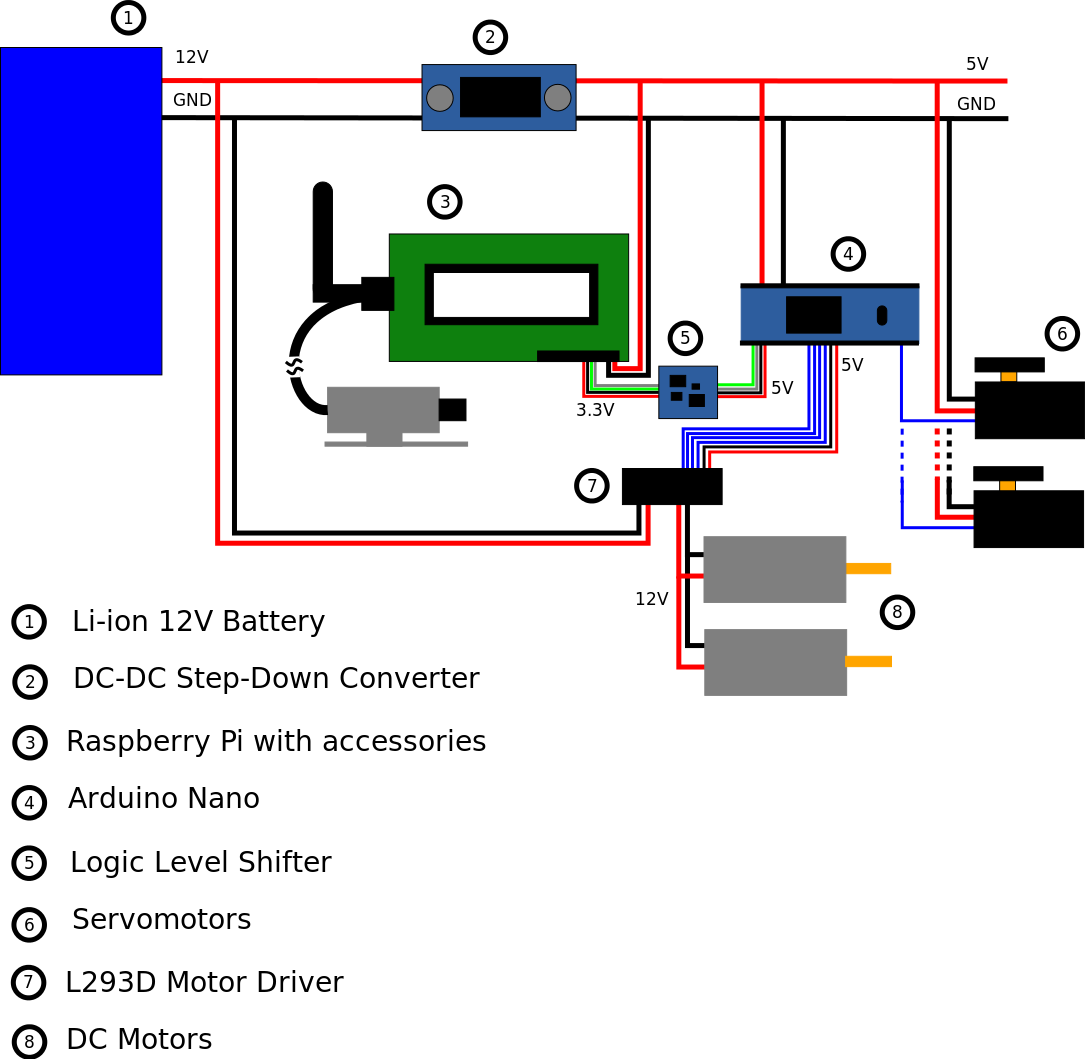
\includegraphics[width=15cm, angle=0]{images/Diagrams/electrical.png}
			\caption{Electrical connections diagram }
			\label{electricDiagram}
	\end{figure}
	\bigskip

%%%%%%%%%% LOGIC %%%%%%%%%%%%%%%%%%%%%%%%%%%%%%%%%%%%%%%%%%%%%%%%%%%%%%%

\subsection{Logic connections}

Figure \ref{logicDiagram} shows how the different components communicate between themselves. As it can be seen, the user controls the robot from the Android application. This implements a bidirectional communication over wifi with the Raspberry Pi, which is used to both send the Raspberry data concerning the movement of the different motors and to receive the video stream from the robot's onboard camera. The Raspberry then communicates over Serial port with the Arduino, which takes care of the data received to obey the user's commands.\\

	\begin{figure}[H]
			\centering
			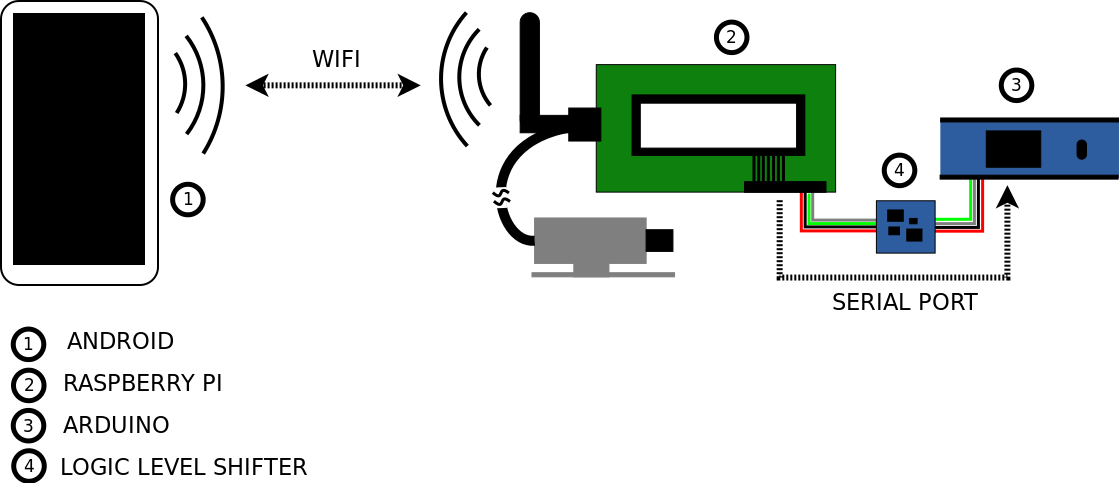
\includegraphics[width=15cm, angle=0]{images/Diagrams/logic.png}
			\caption{Logic connections diagram }
			\label{logicDiagram}
	\end{figure}
	\bigskip